% !TEX encoding = UTF-8 Unicode
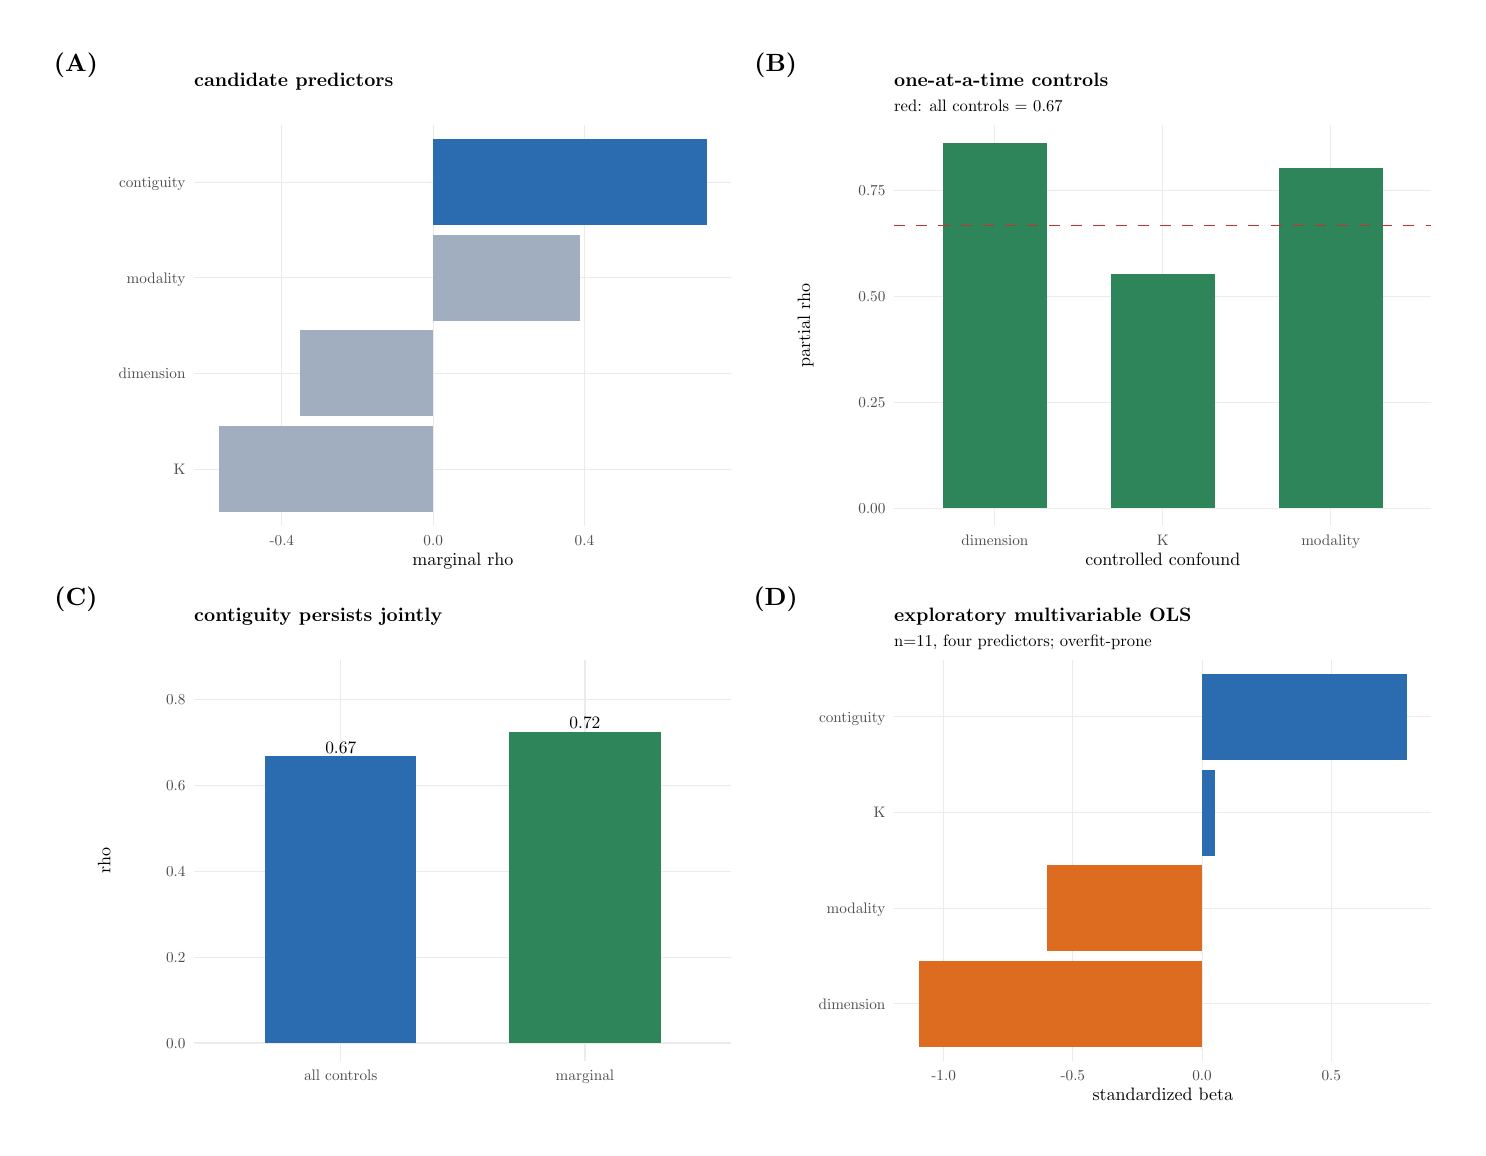
\begin{tikzpicture}[x=1pt,y=1pt]
\definecolor{fillColor}{RGB}{255,255,255}
\path[use as bounding box,fill=fillColor,fill opacity=0.00] (0,0) rectangle (516.73,397.48);
\begin{scope}
\path[clip] (  0.00,  0.00) rectangle (516.73,397.48);
\definecolor{drawColor}{RGB}{255,255,255}
\definecolor{fillColor}{RGB}{255,255,255}

\path[draw=drawColor,line width= 0.6pt,line join=round,line cap=round,fill=fillColor] (  0.00,  0.00) rectangle (516.73,397.48);
\end{scope}
\begin{scope}
\path[clip] (  5.50,198.74) rectangle (258.31,391.98);
\definecolor{fillColor}{RGB}{255,255,255}

\path[fill=fillColor] (  5.50,198.74) rectangle (258.31,391.98);
\end{scope}
\begin{scope}
\path[clip] (258.31,198.74) rectangle (511.23,391.98);
\definecolor{fillColor}{RGB}{255,255,255}

\path[fill=fillColor] (258.31,198.74) rectangle (511.23,391.98);
\end{scope}
\begin{scope}
\path[clip] (  5.50,  5.50) rectangle (258.31,198.74);
\definecolor{fillColor}{RGB}{255,255,255}

\path[fill=fillColor] (  5.50,  5.50) rectangle (258.31,198.74);
\end{scope}
\begin{scope}
\path[clip] (258.31,  5.50) rectangle (511.23,198.74);
\definecolor{fillColor}{RGB}{255,255,255}

\path[fill=fillColor] (258.31,  5.50) rectangle (511.23,198.74);
\end{scope}
\begin{scope}
\path[clip] ( 60.18,217.24) rectangle (254.31,362.39);
\definecolor{drawColor}{gray}{0.92}

\path[draw=drawColor,line width= 0.4pt,line join=round] ( 60.18,237.98) --
	(254.31,237.98);

\path[draw=drawColor,line width= 0.4pt,line join=round] ( 60.18,272.54) --
	(254.31,272.54);

\path[draw=drawColor,line width= 0.4pt,line join=round] ( 60.18,307.10) --
	(254.31,307.10);

\path[draw=drawColor,line width= 0.4pt,line join=round] ( 60.18,341.65) --
	(254.31,341.65);

\path[draw=drawColor,line width= 0.4pt,line join=round] ( 91.84,217.24) --
	( 91.84,362.39);

\path[draw=drawColor,line width= 0.4pt,line join=round] (146.52,217.24) --
	(146.52,362.39);

\path[draw=drawColor,line width= 0.4pt,line join=round] (201.20,217.24) --
	(201.20,362.39);
\definecolor{fillColor}{RGB}{43,108,176}

\path[fill=fillColor] (146.52,326.10) rectangle (245.49,357.21);
\definecolor{fillColor}{RGB}{160,174,192}

\path[fill=fillColor] ( 69.01,222.43) rectangle (146.52,253.53);

\path[fill=fillColor] ( 98.40,256.98) rectangle (146.52,288.09);

\path[fill=fillColor] (146.52,291.54) rectangle (199.69,322.65);
\end{scope}
\begin{scope}
\path[clip] (  0.00,  0.00) rectangle (516.73,397.48);
\definecolor{drawColor}{gray}{0.30}

\node[text=drawColor,anchor=base east,inner sep=0pt, outer sep=0pt, scale=  0.55] at ( 57.03,236.08) {K};

\node[text=drawColor,anchor=base east,inner sep=0pt, outer sep=0pt, scale=  0.55] at ( 57.03,270.64) {dimension};

\node[text=drawColor,anchor=base east,inner sep=0pt, outer sep=0pt, scale=  0.55] at ( 57.03,305.20) {modality};

\node[text=drawColor,anchor=base east,inner sep=0pt, outer sep=0pt, scale=  0.55] at ( 57.03,339.76) {contiguity};
\end{scope}
\begin{scope}
\path[clip] (  0.00,  0.00) rectangle (516.73,397.48);
\definecolor{drawColor}{gray}{0.30}

\node[text=drawColor,anchor=base,inner sep=0pt, outer sep=0pt, scale=  0.55] at ( 91.84,210.30) {-0.4};

\node[text=drawColor,anchor=base,inner sep=0pt, outer sep=0pt, scale=  0.55] at (146.52,210.30) {0.0};

\node[text=drawColor,anchor=base,inner sep=0pt, outer sep=0pt, scale=  0.55] at (201.20,210.30) {0.4};
\end{scope}
\begin{scope}
\path[clip] (  0.00,  0.00) rectangle (516.73,397.48);
\definecolor{drawColor}{RGB}{0,0,0}

\node[text=drawColor,anchor=base,inner sep=0pt, outer sep=0pt, scale=  0.65] at (157.25,203.01) {marginal rho};
\end{scope}
\begin{scope}
\path[clip] (  0.00,  0.00) rectangle (516.73,397.48);
\definecolor{drawColor}{RGB}{0,0,0}

\node[text=drawColor,anchor=base west,inner sep=0pt, outer sep=0pt, scale=  0.70] at ( 60.18,376.05) {\bfseries candidate predictors};
\end{scope}
\begin{scope}
\path[clip] (  0.00,  0.00) rectangle (516.73,397.48);
\definecolor{drawColor}{RGB}{0,0,0}

\node[text=drawColor,anchor=base,inner sep=0pt, outer sep=0pt, scale=  0.90] at ( 17.44,381.82) {\bfseries (A)};
\end{scope}
\begin{scope}
\path[clip] (313.11,217.24) rectangle (507.23,362.39);
\definecolor{drawColor}{gray}{0.92}

\path[draw=drawColor,line width= 0.4pt,line join=round] (313.11,223.84) --
	(507.23,223.84);

\path[draw=drawColor,line width= 0.4pt,line join=round] (313.11,262.15) --
	(507.23,262.15);

\path[draw=drawColor,line width= 0.4pt,line join=round] (313.11,300.47) --
	(507.23,300.47);

\path[draw=drawColor,line width= 0.4pt,line join=round] (313.11,338.78) --
	(507.23,338.78);

\path[draw=drawColor,line width= 0.4pt,line join=round] (349.50,217.24) --
	(349.50,362.39);

\path[draw=drawColor,line width= 0.4pt,line join=round] (410.17,217.24) --
	(410.17,362.39);

\path[draw=drawColor,line width= 0.4pt,line join=round] (470.83,217.24) --
	(470.83,362.39);
\definecolor{fillColor}{RGB}{47,133,90}

\path[fill=fillColor] (391.36,223.84) rectangle (428.97,308.44);

\path[fill=fillColor] (330.70,223.84) rectangle (368.31,355.79);

\path[fill=fillColor] (452.03,223.84) rectangle (489.64,346.60);
\definecolor{drawColor}{RGB}{197,48,48}

\path[draw=drawColor,line width= 0.4pt,dash pattern=on 4pt off 4pt ,line join=round] (313.11,326.06) -- (507.23,326.06);
\end{scope}
\begin{scope}
\path[clip] (  0.00,  0.00) rectangle (516.73,397.48);
\definecolor{drawColor}{gray}{0.30}

\node[text=drawColor,anchor=base east,inner sep=0pt, outer sep=0pt, scale=  0.55] at (309.96,221.95) {0.00};

\node[text=drawColor,anchor=base east,inner sep=0pt, outer sep=0pt, scale=  0.55] at (309.96,260.26) {0.25};

\node[text=drawColor,anchor=base east,inner sep=0pt, outer sep=0pt, scale=  0.55] at (309.96,298.57) {0.50};

\node[text=drawColor,anchor=base east,inner sep=0pt, outer sep=0pt, scale=  0.55] at (309.96,336.89) {0.75};
\end{scope}
\begin{scope}
\path[clip] (  0.00,  0.00) rectangle (516.73,397.48);
\definecolor{drawColor}{gray}{0.30}

\node[text=drawColor,anchor=base,inner sep=0pt, outer sep=0pt, scale=  0.55] at (349.50,210.30) {dimension};

\node[text=drawColor,anchor=base,inner sep=0pt, outer sep=0pt, scale=  0.55] at (410.17,210.30) {K};

\node[text=drawColor,anchor=base,inner sep=0pt, outer sep=0pt, scale=  0.55] at (470.83,210.30) {modality};
\end{scope}
\begin{scope}
\path[clip] (  0.00,  0.00) rectangle (516.73,397.48);
\definecolor{drawColor}{RGB}{0,0,0}

\node[text=drawColor,anchor=base,inner sep=0pt, outer sep=0pt, scale=  0.65] at (410.17,203.01) {controlled confound};
\end{scope}
\begin{scope}
\path[clip] (  0.00,  0.00) rectangle (516.73,397.48);
\definecolor{drawColor}{RGB}{0,0,0}

\node[text=drawColor,rotate= 90.00,anchor=base,inner sep=0pt, outer sep=0pt, scale=  0.65] at (282.77,289.82) {partial rho};
\end{scope}
\begin{scope}
\path[clip] (  0.00,  0.00) rectangle (516.73,397.48);
\definecolor{drawColor}{RGB}{0,0,0}

\node[text=drawColor,anchor=base west,inner sep=0pt, outer sep=0pt, scale=  0.60] at (313.11,367.06) {red: all controls = 0.67};
\end{scope}
\begin{scope}
\path[clip] (  0.00,  0.00) rectangle (516.73,397.48);
\definecolor{drawColor}{RGB}{0,0,0}

\node[text=drawColor,anchor=base west,inner sep=0pt, outer sep=0pt, scale=  0.70] at (313.11,376.05) {\bfseries one-at-a-time controls};
\end{scope}
\begin{scope}
\path[clip] (  0.00,  0.00) rectangle (516.73,397.48);
\definecolor{drawColor}{RGB}{0,0,0}

\node[text=drawColor,anchor=base,inner sep=0pt, outer sep=0pt, scale=  0.90] at (270.30,381.82) {\bfseries (B)};
\end{scope}
\begin{scope}
\path[clip] ( 60.18, 24.00) rectangle (254.31,169.15);
\definecolor{drawColor}{gray}{0.92}

\path[draw=drawColor,line width= 0.4pt,line join=round] ( 60.18, 30.60) --
	(254.31, 30.60);

\path[draw=drawColor,line width= 0.4pt,line join=round] ( 60.18, 61.64) --
	(254.31, 61.64);

\path[draw=drawColor,line width= 0.4pt,line join=round] ( 60.18, 92.69) --
	(254.31, 92.69);

\path[draw=drawColor,line width= 0.4pt,line join=round] ( 60.18,123.74) --
	(254.31,123.74);

\path[draw=drawColor,line width= 0.4pt,line join=round] ( 60.18,154.79) --
	(254.31,154.79);

\path[draw=drawColor,line width= 0.4pt,line join=round] (113.13, 24.00) --
	(113.13,169.15);

\path[draw=drawColor,line width= 0.4pt,line join=round] (201.37, 24.00) --
	(201.37,169.15);
\definecolor{fillColor}{RGB}{47,133,90}

\path[fill=fillColor] (174.01, 30.60) rectangle (228.72,142.99);
\definecolor{fillColor}{RGB}{43,108,176}

\path[fill=fillColor] ( 85.77, 30.60) rectangle (140.48,134.14);
\definecolor{drawColor}{RGB}{0,0,0}

\node[text=drawColor,anchor=base,inner sep=0pt, outer sep=0pt, scale=  0.63] at (201.37,144.07) {0.72};

\node[text=drawColor,anchor=base,inner sep=0pt, outer sep=0pt, scale=  0.63] at (113.13,135.22) {0.67};
\end{scope}
\begin{scope}
\path[clip] (  0.00,  0.00) rectangle (516.73,397.48);
\definecolor{drawColor}{gray}{0.30}

\node[text=drawColor,anchor=base east,inner sep=0pt, outer sep=0pt, scale=  0.55] at ( 57.03, 28.70) {0.0};

\node[text=drawColor,anchor=base east,inner sep=0pt, outer sep=0pt, scale=  0.55] at ( 57.03, 59.75) {0.2};

\node[text=drawColor,anchor=base east,inner sep=0pt, outer sep=0pt, scale=  0.55] at ( 57.03, 90.80) {0.4};

\node[text=drawColor,anchor=base east,inner sep=0pt, outer sep=0pt, scale=  0.55] at ( 57.03,121.85) {0.6};

\node[text=drawColor,anchor=base east,inner sep=0pt, outer sep=0pt, scale=  0.55] at ( 57.03,152.89) {0.8};
\end{scope}
\begin{scope}
\path[clip] (  0.00,  0.00) rectangle (516.73,397.48);
\definecolor{drawColor}{gray}{0.30}

\node[text=drawColor,anchor=base,inner sep=0pt, outer sep=0pt, scale=  0.55] at (113.13, 17.06) {all controls};

\node[text=drawColor,anchor=base,inner sep=0pt, outer sep=0pt, scale=  0.55] at (201.37, 17.06) {marginal};
\end{scope}
\begin{scope}
\path[clip] (  0.00,  0.00) rectangle (516.73,397.48);
\definecolor{drawColor}{RGB}{0,0,0}

\node[text=drawColor,rotate= 90.00,anchor=base,inner sep=0pt, outer sep=0pt, scale=  0.65] at ( 29.85, 96.57) {rho};
\end{scope}
\begin{scope}
\path[clip] (  0.00,  0.00) rectangle (516.73,397.48);
\definecolor{drawColor}{RGB}{0,0,0}

\node[text=drawColor,anchor=base west,inner sep=0pt, outer sep=0pt, scale=  0.70] at ( 60.18,182.81) {\bfseries contiguity persists jointly};
\end{scope}
\begin{scope}
\path[clip] (  0.00,  0.00) rectangle (516.73,397.48);
\definecolor{drawColor}{RGB}{0,0,0}

\node[text=drawColor,anchor=base,inner sep=0pt, outer sep=0pt, scale=  0.90] at ( 17.44,188.58) {\bfseries (C)};
\end{scope}
\begin{scope}
\path[clip] (313.11, 24.00) rectangle (507.23,169.15);
\definecolor{drawColor}{gray}{0.92}

\path[draw=drawColor,line width= 0.4pt,line join=round] (313.11, 44.74) --
	(507.23, 44.74);

\path[draw=drawColor,line width= 0.4pt,line join=round] (313.11, 79.29) --
	(507.23, 79.29);

\path[draw=drawColor,line width= 0.4pt,line join=round] (313.11,113.85) --
	(507.23,113.85);

\path[draw=drawColor,line width= 0.4pt,line join=round] (313.11,148.41) --
	(507.23,148.41);

\path[draw=drawColor,line width= 0.4pt,line join=round] (330.99, 24.00) --
	(330.99,169.15);

\path[draw=drawColor,line width= 0.4pt,line join=round] (377.67, 24.00) --
	(377.67,169.15);

\path[draw=drawColor,line width= 0.4pt,line join=round] (424.36, 24.00) --
	(424.36,169.15);

\path[draw=drawColor,line width= 0.4pt,line join=round] (471.05, 24.00) --
	(471.05,169.15);
\definecolor{fillColor}{RGB}{43,108,176}

\path[fill=fillColor] (424.36,132.86) rectangle (498.41,163.96);

\path[fill=fillColor] (424.36, 98.30) rectangle (429.12,129.40);
\definecolor{fillColor}{RGB}{221,107,32}

\path[fill=fillColor] (321.93, 29.18) rectangle (424.36, 60.29);

\path[fill=fillColor] (368.34, 63.74) rectangle (424.36, 94.85);
\end{scope}
\begin{scope}
\path[clip] (  0.00,  0.00) rectangle (516.73,397.48);
\definecolor{drawColor}{gray}{0.30}

\node[text=drawColor,anchor=base east,inner sep=0pt, outer sep=0pt, scale=  0.55] at (309.96, 42.84) {dimension};

\node[text=drawColor,anchor=base east,inner sep=0pt, outer sep=0pt, scale=  0.55] at (309.96, 77.40) {modality};

\node[text=drawColor,anchor=base east,inner sep=0pt, outer sep=0pt, scale=  0.55] at (309.96,111.96) {K};

\node[text=drawColor,anchor=base east,inner sep=0pt, outer sep=0pt, scale=  0.55] at (309.96,146.52) {contiguity};
\end{scope}
\begin{scope}
\path[clip] (  0.00,  0.00) rectangle (516.73,397.48);
\definecolor{drawColor}{gray}{0.30}

\node[text=drawColor,anchor=base,inner sep=0pt, outer sep=0pt, scale=  0.55] at (330.99, 17.06) {-1.0};

\node[text=drawColor,anchor=base,inner sep=0pt, outer sep=0pt, scale=  0.55] at (377.67, 17.06) {-0.5};

\node[text=drawColor,anchor=base,inner sep=0pt, outer sep=0pt, scale=  0.55] at (424.36, 17.06) {0.0};

\node[text=drawColor,anchor=base,inner sep=0pt, outer sep=0pt, scale=  0.55] at (471.05, 17.06) {0.5};
\end{scope}
\begin{scope}
\path[clip] (  0.00,  0.00) rectangle (516.73,397.48);
\definecolor{drawColor}{RGB}{0,0,0}

\node[text=drawColor,anchor=base,inner sep=0pt, outer sep=0pt, scale=  0.65] at (410.17,  9.76) {standardized beta};
\end{scope}
\begin{scope}
\path[clip] (  0.00,  0.00) rectangle (516.73,397.48);
\definecolor{drawColor}{RGB}{0,0,0}

\node[text=drawColor,anchor=base west,inner sep=0pt, outer sep=0pt, scale=  0.60] at (313.11,173.81) {n=11, four predictors; overfit-prone};
\end{scope}
\begin{scope}
\path[clip] (  0.00,  0.00) rectangle (516.73,397.48);
\definecolor{drawColor}{RGB}{0,0,0}

\node[text=drawColor,anchor=base west,inner sep=0pt, outer sep=0pt, scale=  0.70] at (313.11,182.81) {\bfseries exploratory multivariable OLS};
\end{scope}
\begin{scope}
\path[clip] (  0.00,  0.00) rectangle (516.73,397.48);
\definecolor{drawColor}{RGB}{0,0,0}

\node[text=drawColor,anchor=base,inner sep=0pt, outer sep=0pt, scale=  0.90] at (270.30,188.58) {\bfseries (D)};
\end{scope}
\end{tikzpicture}
